\documentclass[../Main.tex]{subfiles}
\begin{document}
Given the distinctive characteristics of the system discussed in Chapter 3, it is essential to adopt an architecture or combination of multiple architectures to efficiently address these specific requirements while ensuring scalability, reliability, and seamless communication between different components. This chapter aims to deliver an in-depth exploration of the architecture design implemented in the project and provide a detailed understanding of each element in the system.
\section{Architecture design}
\subsection{Software architecture selection}
\begin{figure}[H]
    \centering
    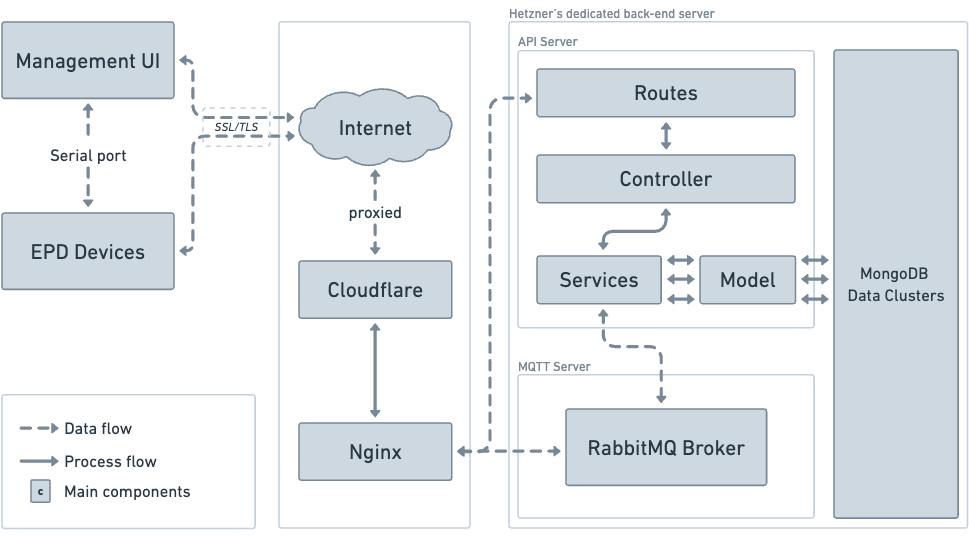
\includegraphics[scale=0.46]{doc/thesis/EN/imgs/overall-architecture.png}
    \caption{Overall architecture of the system}
    \label{fig:Fig1}
\end{figure}

\textbf{Figure \ref{fig:Fig1}} illustrates the system's general architecture and provides an overview of its data flow. The system strategically uses the combination of MVCS (Model-View-Controller-Service) and microservice architectures to take advantage of their unique strengths in specific aspects. This hybrid architecture leverages the benefits of both architectural styles, such as scalability, flexibility, and the ability to use different technologies and patterns within each service.

Microservices architecture is a software development method that structures an application as a collection of loosely coupled services. In this architecture, each service can be developed, deployed, and scaled independently, allowing greater scalability, flexibility, and agility than monolithic architectures, as teams can update or fix individual components without impacting the entire system in case of failure. Thanks to its ability to accommodate the dynamic and distributed natures of IoT applications, microservice architecture is frequently used in various IoT projects. It allows organizations to build more agile and adaptive applications to handle the complex demands of modern business environments.

On the other hand, the Model-View-Controller-Service (MVCS) architecture is an extension of the traditional Model-View-Controller (MVC) pattern. It introduces a service layer sitting between the Controller and the Model, responsible for containing business logic and rules. This layer abstracts complex business operations, allowing Controllers to focus on handling incoming requests and delegating the heavy lifting to Services. This design pattern is well-suited to many web applications and provides a structured and organized approach to developing complex applications, making it easier to manage, maintain, and scale the system over time.

By combining these two architectures, the system is better equipped to handle the dynamic and distributed nature of IoT applications. It also enables organizations to build more agile and adaptive applications to address the complex demands of modern business environments while ensuring scalability, reliability, and seamless communication between different components.

\subsection{Overall design}
The system is divided into independently deployable services, including the API back-end server and MQTT Server. These services communicate via the MQTT protocol, and the MQTT Server also acts as a broker to relay data to the EPD devices (Figure \ref{fig:Fig3}). API server follows the MVCS pattern with three main components: Controllers handling incoming requests and coordinating responses, Services containing the business logic and rules of the application, and Models interacting with the database, managing data storage and retrieval, while Management UI and EPD devices act as a View component (Figure \ref{fig:Fig2}).
\subsubsection{MVCS architecture}
The system has three data types, and the packages of each type handling operation share the same structure: the Controller handles requests about the data type and delegates them to the Service, which processes the requests and uses the Model to interact with the database.
\begin{figure}[H]
    \centering
    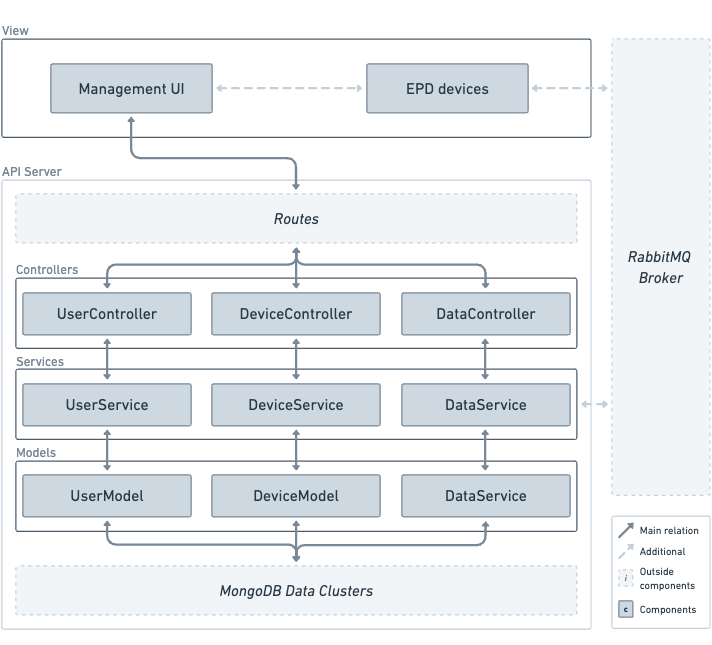
\includegraphics[scale=0.6]{doc/thesis/EN/imgs/api-server.png}
    \caption{MVCS architecture}
    \label{fig:Fig2}
\end{figure}

\subsubsection{MQTT Server}
This service in the system acts as an intermediary, managing the state of all MQTT client connections, subscriptions, and message exchanges.
\begin{figure}[H]
    \centering
    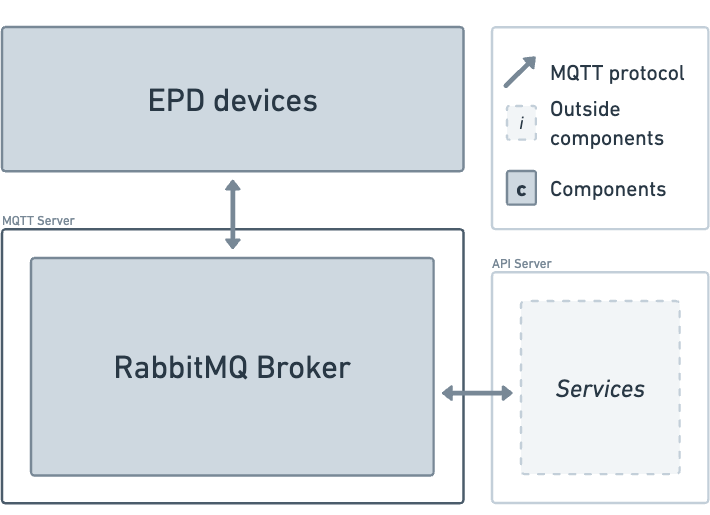
\includegraphics[scale=0.3]{doc/thesis/EN/imgs/mqtt-server.png}
    \caption{MQTT microservice}
    \label{fig:Fig3}
\end{figure}

\subsection{Detailed package design}
\subsubsection{Models}
\begin{figure}[htbp]
    \centering
    \begin{tikzpicture}[]
         \begin{umlpackage}{Models}
            \umlclass[x = 3, y = 8, scale = 0.6]{UserModel}{
                email: string \\
                password: string \\
                name: string \\
                gender: string \\
                \_id: ObjectId \\
                createdAt: time \\
                updatedAt: time
            }{
                \umlvirt{UserModel(userModel: dict): UserModel} \\
                findByIdAndUpdate(id: string): UserModel \\
                findById(id: string): UserModel \\
                findByIdAndRemove(id: string): void \\
                create(data: dict): UserModel \\
                findOne(filter: dict): UserModel
            }

            \umlclass[x = 0, y = 0, scale = 0.6]{DeviceModel}{
                \_id: ObjectId \\
                name: string \\
                ssid: string \\
                pass: string \\
                dataID: ObjectId \\
                dataName: string \\
                active: boolean \\
                createdBy: ObjectId \\
            }{
                \umlvirt{DeviceModel(deviceModel: dict): DeviceModel} \\
                findByIdAndUpdate(id: string): DeviceModel \\
                findById(id: string): DeviceModel \\
                findByIdAndRemove(id: string): void \\
                create(data: dict): DeviceModel \\
                findOne(filter: dict): DeviceModel \\
                find(filter: dict): Array(DeviceModel)
            }
            
            \umlclass[x = 7, y = 0, scale = 0.6]{DataModel}{
                \_id: ObjectId \\
                type: string \\
                name: string \\
                input2: string \\
                input3: string \\
                active: boolean \\
                activeStartTime: uint \\
                deviceID: ObjectId \\
                deviceName: string \\
                activeTimestamp: Array \\
                fontStyle: string \\
                designSchema: string \\
                createdBy: ObjectId
            }{
                \umlvirt{DataModel(deviceModel: dict): DataModel} \\
                findByIdAndUpdate(id: string): DataModel \\
                findById(id: string): DataModel \\
                findByIdAndRemove(id: string): void \\
                create(data: dict): DataModel \\
                findOne(filter: dict): DataModel
            }
            
            \umlassoc[mult1=1, mult2=*, pos1=0.03, pos2=0.8, align1=left, align2=left]{UserModel}{DeviceModel}
            \umlassoc[mult1=1, mult2=*, pos1=0.03, pos2=0.8, align1=right, align2=right]{UserModel}{DataModel}

            % Bidirectional Dependency
            \umldashedline{DeviceModel}{DataModel}
            \umldep[arg=updates, pos=0.5]{DeviceModel}{DataModel}
            \umldep[pos=0.5]{DataModel}{DeviceModel}
         \end{umlpackage}
    \end{tikzpicture}
    \caption{General use case diagram of the data management system}
    \label{fig:ModelClassDiagram}
\end{figure}
\subsubsection{Services}
\begin{figure}[htbp]
    \centering
    \begin{tikzpicture}[]
         \begin{umlpackage}{Services}
            \umlclass[x = 3, y = 3, scale = 0.6]{UserService}{}{
                findUserByEmail(email: string): UserModel \\
                createUser(user: dict): UserModel \\
                getUserById(id: string): UserModel \\
                updateUser(id: string, user: dict): UserModel \\
            }

            \umlclass[x = 0, y = 0, scale = 0.6]{DeviceService}{}{
                getAllDevices(filter: dict): Array(DeviceModel) \\
                getDeviceById(id: string): DeviceModel \\
                createDevice(data: dict, userId: string): DeviceModel \\
                updateDevice(id: string, data: dict): DeviceModel \\
                deleteDevice(id: string, userId: string): void
            }
            
            \umlclass[x = 6, y = 0, scale = 0.6]{DataService}{}{
                findDataByEmail(email: string): DataModel \\
                getAllDatas(filter: dict): Array(DataModel) \\
                getDataById(id: string): DataModel \\
                createData(data: dict, userId: string): DataModel \\
                updateData(id: string, data: dict): DataModel \\
                deleteData(id: string, userId: string): void
            }
         \end{umlpackage}
    \end{tikzpicture}
    \caption{General use case diagram of the data management system}
    \label{fig:ServiceClassDiagram}
\end{figure}

\subsubsection{Controllers}
\begin{figure}[htbp]
    \centering
    \begin{tikzpicture}[]
         \begin{umlpackage}{Controllers}
            \umlclass[x = 3, y = 3, scale = 0.6]{UserController}{
                userService: UserService
            }{
                register(): void \\
                login(id: string): void \\
                getAccountById(): UserModel \\
                updateAccount(): UserModel
            }

            \umlclass[x = 0, y = 0, scale = 0.6]{DeviceController}{
                deviceService: DeviceService
            }{
                
                getAllDevices(): Array(DeviceModel) \\
                createDevice(): DeviceModel \\
                getDeviceById(): DeviceModel \\
                updateDevice(): DeviceModel \\
                deleteDevice(): void
            }
            
            \umlclass[x = 5, y = 0, scale = 0.6]{DataController}{
                dataService: DataService
            }{
                getAllData(): Array(DataModel) \\
                createData(): DataModel \\
                getDataById(): DataModel \\
                updateData(): DataModel \\
                deleteData(): void
            }
            
         \end{umlpackage}
    \end{tikzpicture}
    \caption{General use case diagram of the data management system}
    \label{fig:DataClassDiagram}
\end{figure}

\subsubsection{Views}
\begin{figure}[htbp]
    \centering
    \begin{tikzpicture}[]
         \begin{umlpackage}{Views}
            \umlclass[x = -1, y = 3, scale = 0.6]{AccountView}{}{
                handleSubmit(e: event): void \\
            }
            
            \umlclass[x = 2.6, y = 3, scale = 0.6]{NewDeviceView}{}{
                connectESP(): void \\
                handleSubmit(e: event): void \\
                handleReset(): void
            }

            \umlclass[x = 6.2, y = 3, scale = 0.6]{DeviceView}{}{
                connectESP(): void \\
                deleteItem(): void \\
                handleSubmit(e: event): void \\
                handleReset(): void
            }
            
            \umlclass[x = 0, y = 0.7, scale = 0.6]{NewDataView}{}{
                handleStage(e: event): void \\
                handleSubmit(e: event): void \\
                handleReset(): void \\
                getActiveDevices(): Array(DeviceModel)
            }

            \umlclass[x = 5, y = 1, scale = 0.6]{DataView}{}{
                handleSubmit(e: event): void \\
                getActiveDevices(): Array(DeviceModel)
            }
         \end{umlpackage}
    \end{tikzpicture}
    \caption{General use case diagram of the data management system}
    \label{fig:DataClassDiagram}
\end{figure}


\section{Detailed design}
\subsection{User interface design}
The architecture and user interface of this system are meticulously tailored for computer displays, ensuring optimal functionality and visual experience on larger screens. The design is customized to leverage the expansive real estate of computer monitors, facilitating ease of use and comprehensive display of information. This focus on computer-targeted design means that the system is not intended for mobile use, and as such, it may not provide an ideal user experience or full functionality on smaller, mobile device screens. The decision to specialize in computer displays stems from a commitment to delivering a high-quality, immersive experience that fully utilizes the capabilities and advantages of larger screens typically associated with desktop or laptop computers.
\begin{figure}[H]
    \centering
    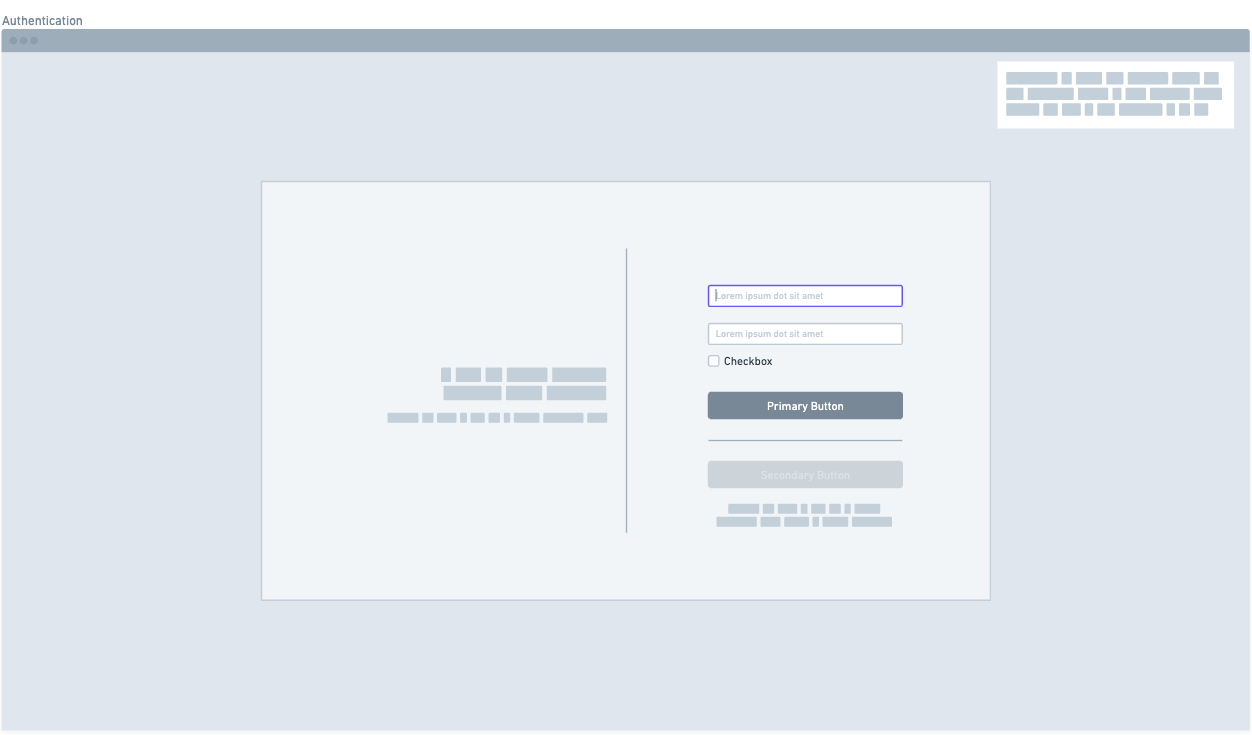
\includegraphics[scale=0.35]{doc/thesis/EN/imgs/mockup1.png}
    \caption{Mockup display of authentication page}
    \label{fig:Mockup1}
\end{figure}
\begin{figure}[H]
    \centering
    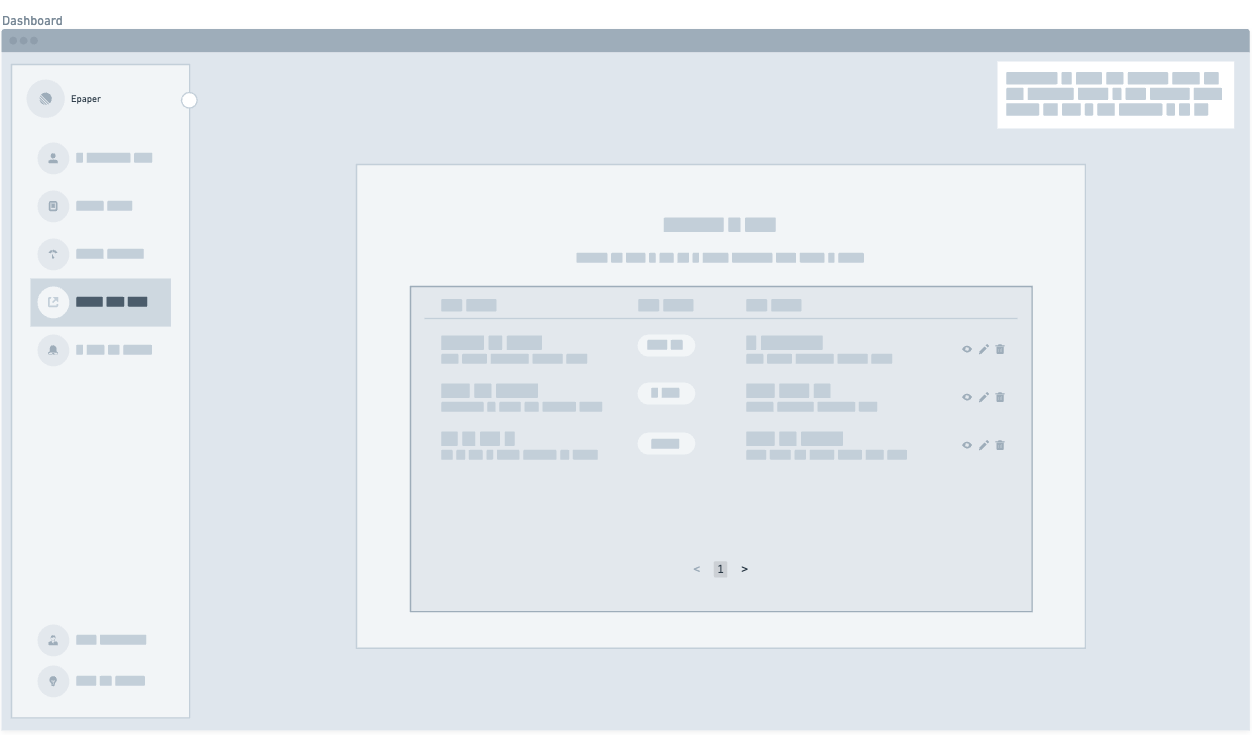
\includegraphics[scale=0.35]{doc/thesis/EN/imgs/mockup2.png}
    \caption{Mockup display of dashboard page}
    \label{fig:Mockup2}
\end{figure}
\begin{figure}[H]
    \centering
    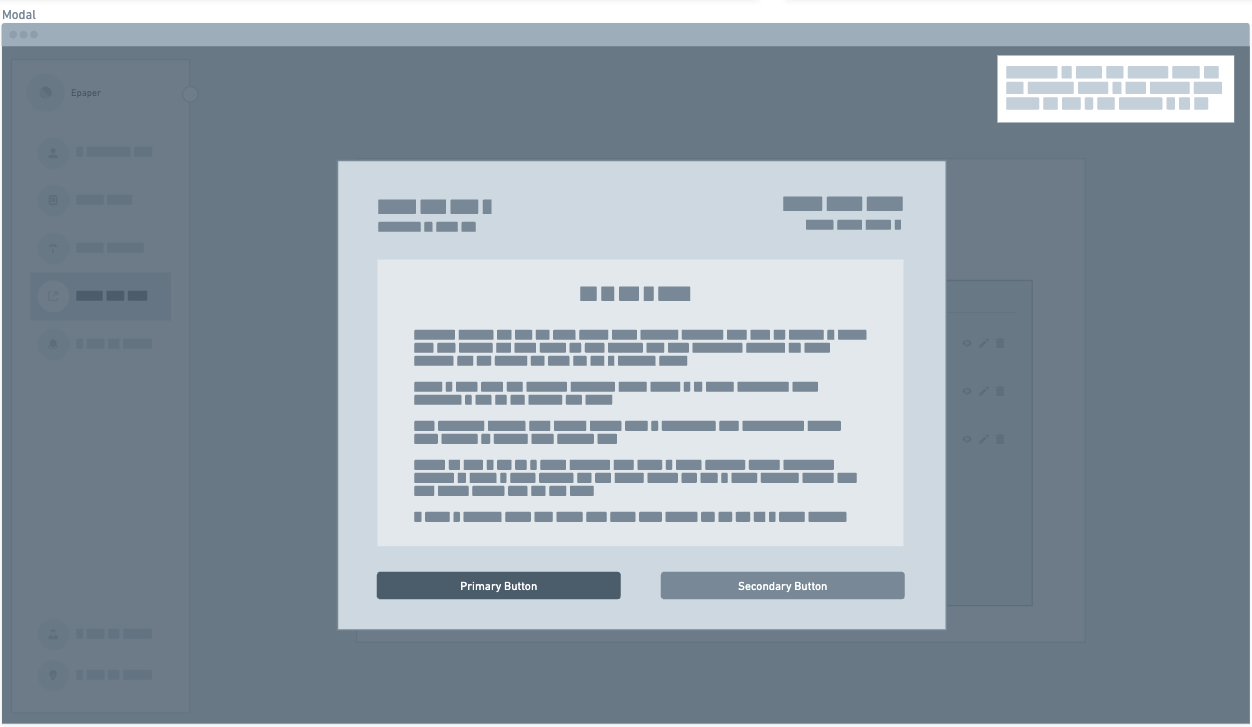
\includegraphics[scale=0.35]{doc/thesis/EN/imgs/mockup3.png}
    \caption{Mockup display of modal component}
    \label{fig:Mockup3}
\end{figure}
\begin{figure}[H]
    \centering
    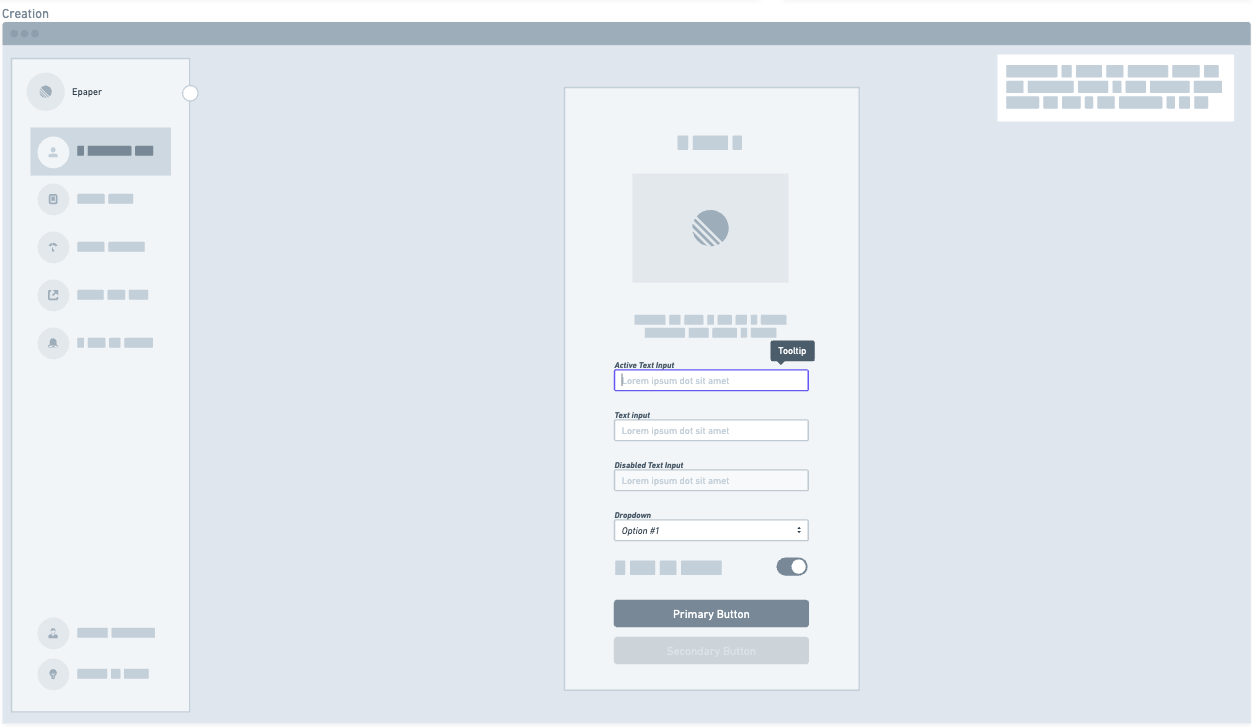
\includegraphics[scale=0.35]{doc/thesis/EN/imgs/mockup4.png}
    \caption{Mockup display of creation page}
    \label{fig:Mockup4}
\end{figure}

\subsection{Layer design}
Each sub-section below demonstrates the workflow of each class participating in each use case in form of class diagram, and a responding sequence diagram.
\subsubsection{Class and sequence diagram of use case "Register a new device"}
\begin{figure}[htbp]
    \centering
    \begin{tikzpicture}
        % \draw (-1.5, 2.5) rectangle (13, -8);
    
        % Define system boundary
        \umlactor[x = -0.5, y = 4, scale = 0.8]{Manager}
        \umlactor[x = 2.5, y = 5, scale = 0.8]{EPD Devices}
        
        \begin{umlpackage}{pkg}
            \umlclass[x = 0, y = 8, scale = 0.5]{NewDeviceView}{}{
                connectESP(): void \\
                handleSubmit(e: event): void \\
                handleReset(): void
            }
            
            \umlclass[x = 5, y = 8, scale = 0.5]{DeviceController}{
                deviceService: DeviceService
            }{
                getAllDevices(): Array(DeviceModel) \\
                createDevice(): DeviceModel \\
                getDeviceById(): DeviceModel \\
                updateDevice(): DeviceModel \\
                deleteDevice(): void
            }

            \umlclass[x = 5, y = 2, scale = 0.5]{DeviceService}{}{
                getAllDevices(filter: dict): Array(DeviceModel) \\
                getDeviceById(id: string): DeviceModel \\
                createDevice(data: dict, userId: string): DeviceModel \\
                updateDevice(id: string, data: dict): DeviceModel \\
                deleteDevice(id: string, userId: string): void
            }

            \umlclass[x = 10, y = 6, scale = 0.5]{DeviceModel}{
                \_id: ObjectId \\
                name: string \\
                ssid: string \\
                pass: string \\
                dataID: ObjectId \\
                dataName: string \\
                active: boolean \\
                createdBy: ObjectId \\
            }{
                \umlvirt{DeviceModel(deviceModel: dict): DeviceModel} \\
                findByIdAndUpdate(id: string): DeviceModel \\
                findById(id: string): DeviceModel \\
                findByIdAndRemove(id: string): void \\
                create(data: dict): DeviceModel \\
                findOne(filter: dict): DeviceModel \\
                find(filter: dict): Array(DeviceModel)
            }
        \end{umlpackage}
        
        \umluniassoc[]{Manager}{NewDeviceView}
        \umluniassoc[]{NewDeviceView}{EPD Devices}
        \umluniassoc[geometry = |-, anchor1 = 100, anchor2 = 0]{DeviceService}{EPD Devices}
        \umluniassoc[]{NewDeviceView}{DeviceController}
        \umluniassoc[]{DeviceController}{DeviceService}
        \umluniassoc[]{DeviceService}{DeviceModel}
    \end{tikzpicture}
    \caption{Detailed use case of Data Management function}
    \label{fig:usecasediagram}
\end{figure}

\subsubsection{Class and sequence diagram of use case "Add a new data"}
\begin{figure}[htbp]
    \centering
    \begin{tikzpicture}
        % Define system boundary
        \umlactor[x = 3, y = 10, scale = 0.7]{Manager}
        \umlactor[x = 6, y = 5, scale = 0.7]{EPD Devices}
        
        \begin{umlpackage}{pkg}
            \umlclass[x = 8, y = 10, scale = 0.5]{NewDataView}{}{
                handleStage(e: event): void \\
                handleSubmit(e: event): void \\
                handleReset(): void \\
                getActiveDevices(): Array(DeviceModel)
            }

            \umlclass[x = 4, y = 7, scale = 0.5]{DataController}{
                dataService: DataService
            }{
                getAllData(): Array(DataModel) \\
                createData(): DataModel \\
                getDataById(): DataModel \\
                updateData(): DataModel \\
                deleteData(): void
            }

            \umlclass[x = 9, y = 7, scale = 0.5]{DeviceController}{
                deviceService: DeviceService
            }{
                getAllDevices(): Array(DeviceModel) \\
                createDevice(): DeviceModel \\
                getDeviceById(): DeviceModel \\
                updateDevice(): DeviceModel \\
                deleteDevice(): void
            }

            \umlclass[x = 4, y = 2, scale = 0.5]{DataService}{}{
                findDataByEmail(email: string): DataModel \\
                getAllDatas(filter: dict): Array(DataModel) \\
                getDataById(id: string): DataModel \\
                createData(data: dict, userId: string): DataModel \\
                updateData(id: string, data: dict): DataModel \\
                deleteData(id: string, userId: string): void
            }

            \umlclass[x = 9, y = 2, scale = 0.5]{DeviceService}{}{
                getAllDevices(filter: dict): Array(DeviceModel) \\
                getDeviceById(id: string): DeviceModel \\
                createDevice(data: dict, userId: string): DeviceModel \\
                updateDevice(id: string, data: dict): DeviceModel \\
                deleteDevice(id: string, userId: string): void
            }

            \umlclass[x = 14, y = 2, scale = 0.5]{DeviceModel}{
                \_id: ObjectId \\
                name: string \\
                ssid: string \\
                pass: string \\
                dataID: ObjectId \\
                dataName: string \\
                active: boolean \\
                createdBy: ObjectId \\
            }{
                \umlvirt{DeviceModel(deviceModel: dict): DeviceModel} \\
                findByIdAndUpdate(id: string): DeviceModel \\
                findById(id: string): DeviceModel \\
                findByIdAndRemove(id: string): void \\
                create(data: dict): DeviceModel \\
                findOne(filter: dict): DeviceModel \\
                find(filter: dict): Array(DeviceModel)
            }
            
            \umlclass[x = 14, y = 7.5, scale = 0.5]{DataModel}{
                \_id: ObjectId \\
                type: string \\
                name: string \\
                input2: string \\
                input3: string \\
                active: boolean \\
                activeStartTime: uint \\
                deviceID: ObjectId \\
                deviceName: string \\
                activeTimestamp: Array \\
                fontStyle: string \\
                designSchema: string \\
                createdBy: ObjectId
            }{
                \umlvirt{DataModel(deviceModel: dict): DataModel} \\
                findByIdAndUpdate(id: string): DataModel \\
                findById(id: string): DataModel \\
                findByIdAndRemove(id: string): void \\
                create(data: dict): DataModel \\
                findOne(filter: dict): DataModel
            }
        \end{umlpackage}
        
        \umluniassoc[]{Manager}{NewDataView}
        \umluniassoc[geometry = |-, anchor1 = 80, anchor2 = -180]{DataService}{EPD Devices}
        \umluniassoc[geometry = |-, anchor1 = 100, anchor2 = 0]{DeviceService}{EPD Devices}
        \umluniassoc[]{NewDataView}{DataController}
        \umluniassoc[]{NewDataView}{DeviceController}
        \umluniassoc[]{DataController}{DataService}
        \umluniassoc[]{DeviceController}{DeviceService}
        \umluniassoc[]{DataService}{DataModel}
        \umluniassoc[geometry = |-, anchor1 = -90, anchor2 = -140]{DataService}{DeviceModel}
        \umluniassoc[]{DeviceService}{DeviceModel}
    \end{tikzpicture}
    \caption{Detailed use case of Data Management function}
    \label{fig:usecasediagram}
\end{figure}

\subsubsection{Class and sequence diagram of use case "Change a device information"}
\begin{figure}[htbp]
    \centering
    \begin{tikzpicture}
        % Define system boundary
        \umlactor[x = 3, y = 10, scale = 0.7]{Manager}
        \umlactor[x = 5.5, y = 5, scale = 0.7]{EPD Devices}

        \begin{umlpackage}{pkg}
            \umlclass[x = 8, y = 10, scale = 0.5]{DeviceView}{}{
                connectESP(): void \\
                deleteItem(): void \\
                handleSubmit(e: event): void \\
                handleReset(): void
            }

            \umlclass[x = 9, y = 7, scale = 0.5]{DeviceController}{
                deviceService: DeviceService
            }{
                getAllDevices(): Array(DeviceModel) \\
                createDevice(): DeviceModel \\
                getDeviceById(): DeviceModel \\
                updateDevice(): DeviceModel \\
                deleteDevice(): void
            }

            \umlclass[x = 4, y = 2, scale = 0.5]{DataService}{}{
                findDataByEmail(email: string): DataModel \\
                getAllDatas(filter: dict): Array(DataModel) \\
                getDataById(id: string): DataModel \\
                createData(data: dict, userId: string): DataModel \\
                updateData(id: string, data: dict): DataModel \\
                deleteData(id: string, userId: string): void
            }

            \umlclass[x = 9, y = 2, scale = 0.5]{DeviceService}{}{
                getAllDevices(filter: dict): Array(DeviceModel) \\
                getDeviceById(id: string): DeviceModel \\
                createDevice(data: dict, userId: string): DeviceModel \\
                updateDevice(id: string, data: dict): DeviceModel \\
                deleteDevice(id: string, userId: string): void
            }

            \umlclass[x = 14, y = 2, scale = 0.5]{DeviceModel}{
                \_id: ObjectId \\
                name: string \\
                ssid: string \\
                pass: string \\
                dataID: ObjectId \\
                dataName: string \\
                active: boolean \\
                createdBy: ObjectId \\
            }{
                \umlvirt{DeviceModel(deviceModel: dict): DeviceModel} \\
                findByIdAndUpdate(id: string): DeviceModel \\
                findById(id: string): DeviceModel \\
                findByIdAndRemove(id: string): void \\
                create(data: dict): DeviceModel \\
                findOne(filter: dict): DeviceModel \\
                find(filter: dict): Array(DeviceModel)
            }
            
            \umlclass[x = 14, y = 7.5, scale = 0.5]{DataModel}{
                \_id: ObjectId \\
                type: string \\
                name: string \\
                input2: string \\
                input3: string \\
                active: boolean \\
                activeStartTime: uint \\
                deviceID: ObjectId \\
                deviceName: string \\
                activeTimestamp: Array \\
                fontStyle: string \\
                designSchema: string \\
                createdBy: ObjectId
            }{
                \umlvirt{DataModel(deviceModel: dict): DataModel} \\
                findByIdAndUpdate(id: string): DataModel \\
                findById(id: string): DataModel \\
                findByIdAndRemove(id: string): void \\
                create(data: dict): DataModel \\
                findOne(filter: dict): DataModel
            }
        \end{umlpackage}
        
        \umluniassoc[]{Manager}{DeviceView}
        \umluniassoc[geometry = |-, anchor1 = 100, anchor2 = 0]{DeviceService}{EPD Devices}
        \umluniassoc[]{DeviceView}{EPD Devices}
        \umluniassoc[]{DeviceView}{DataController}
        \umluniassoc[]{DeviceView}{DeviceController}
        \umluniassoc[]{DataController}{DataService}
        \umluniassoc[]{DeviceController}{DeviceService}
        \umluniassoc[]{DataService}{DataModel}
        \umluniassoc[geometry = |-, anchor1 = 80, anchor2 = -130]{DeviceService}{DataModel}
        \umluniassoc[]{DeviceService}{DeviceModel}
    \end{tikzpicture}
    \caption{Detailed use case of Data Management function}
    \label{fig:usecasediagram}
\end{figure}
\subsubsection{Class and sequence diagram of use case "Change data information"}
\begin{figure}[htbp]
    \centering
    \begin{tikzpicture}
        % Define system boundary
        \umlactor[x = 3, y = 10, scale = 0.7]{Manager}
        \umlactor[x = 5.5, y = 5, scale = 0.7]{EPD Devices}
        
        \begin{umlpackage}{pkg}
            \umlclass[x = 8, y = 10, scale = 0.5]{DataView}{}{
                handleSubmit(e: event): void \\
                getActiveDevices(): Array(DeviceModel)
            }

            \umlclass[x = 4, y = 7, scale = 0.5]{DataController}{
                dataService: DataService
            }{
                getAllData(): Array(DataModel) \\
                createData(): DataModel \\
                getDataById(): DataModel \\
                updateData(): DataModel \\
                deleteData(): void
            }

            \umlclass[x = 9, y = 7, scale = 0.5]{DeviceController}{
                deviceService: DeviceService
            }{
                getAllDevices(): Array(DeviceModel) \\
                createDevice(): DeviceModel \\
                getDeviceById(): DeviceModel \\
                updateDevice(): DeviceModel \\
                deleteDevice(): void
            }

            \umlclass[x = 4, y = 2, scale = 0.5]{DataService}{}{
                findDataByEmail(email: string): DataModel \\
                getAllDatas(filter: dict): Array(DataModel) \\
                getDataById(id: string): DataModel \\
                createData(data: dict, userId: string): DataModel \\
                updateData(id: string, data: dict): DataModel \\
                deleteData(id: string, userId: string): void
            }

            \umlclass[x = 9, y = 2, scale = 0.5]{DeviceService}{}{
                getAllDevices(filter: dict): Array(DeviceModel) \\
                getDeviceById(id: string): DeviceModel \\
                createDevice(data: dict, userId: string): DeviceModel \\
                updateDevice(id: string, data: dict): DeviceModel \\
                deleteDevice(id: string, userId: string): void
            }

            \umlclass[x = 14, y = 2, scale = 0.5]{DeviceModel}{
                \_id: ObjectId \\
                name: string \\
                ssid: string \\
                pass: string \\
                dataID: ObjectId \\
                dataName: string \\
                active: boolean \\
                createdBy: ObjectId \\
            }{
                \umlvirt{DeviceModel(deviceModel: dict): DeviceModel} \\
                findByIdAndUpdate(id: string): DeviceModel \\
                findById(id: string): DeviceModel \\
                findByIdAndRemove(id: string): void \\
                create(data: dict): DeviceModel \\
                findOne(filter: dict): DeviceModel \\
                find(filter: dict): Array(DeviceModel)
            }
            
            \umlclass[x = 14, y = 7.5, scale = 0.5]{DataModel}{
                \_id: ObjectId \\
                type: string \\
                name: string \\
                input2: string \\
                input3: string \\
                active: boolean \\
                activeStartTime: uint \\
                deviceID: ObjectId \\
                deviceName: string \\
                activeTimestamp: Array \\
                fontStyle: string \\
                designSchema: string \\
                createdBy: ObjectId
            }{
                \umlvirt{DataModel(deviceModel: dict): DataModel} \\
                findByIdAndUpdate(id: string): DataModel \\
                findById(id: string): DataModel \\
                findByIdAndRemove(id: string): void \\
                create(data: dict): DataModel \\
                findOne(filter: dict): DataModel
            }
        \end{umlpackage}
        
        \umluniassoc[]{Manager}{DataView}
        \umluniassoc[geometry = |-, anchor1 = 80, anchor2 = -180]{DataService}{EPD Devices}
        \umluniassoc[geometry = |-, anchor1 = 100, anchor2 = 0]{DeviceService}{EPD Devices}
        \umluniassoc[]{DataView}{DataController}
        \umluniassoc[]{DataView}{DeviceController}
        \umluniassoc[]{DataController}{DataService}
        \umluniassoc[]{DeviceController}{DeviceService}
        \umluniassoc[]{DataService}{DataModel}
        \umluniassoc[geometry = |-, anchor1 = -90, anchor2 = -140]{DataService}{DeviceModel}
        \umluniassoc[]{DeviceService}{DeviceModel}
    \end{tikzpicture}
    \caption{Detailed use case of Data Management function}
    \label{fig:usecasediagram}
\end{figure}
\subsubsection{Class and sequence diagram of use case "Remove a device"}
\subsubsection{Class and sequence diagram of use case "Remove a data"}
\subsubsection{Class and sequence diagram of use case "Register new account"}
\subsubsection{Class and sequence diagram of use case "Sign in"}

\subsection{Database design}
Phần này có độ dài từ hai đến bốn trang. Sinh viên thiết kế, vẽ và giải thích biểu đồ thực thể liên kết (E-R diagram). Từ đó, sinh viên thiết kế cơ sở dữ liệu tùy theo hệ quản trị cơ sở dữ liệu mà mình sử dụng (SQL, NoSQL, Firebase, v.v.)

\section{Application Building}
\subsection{Libraries and Tools}
Sinh viên liệt kê các công cụ, ngôn ngữ lập trình, API, thư viện, IDE, công cụ kiểm thử, v.v. mà mình sử dụng để phát triển ứng dụng. Mỗi công cụ phải được chỉ rõ phiên bản sử dụng. SV nên kẻ bảng mô tả tương tự như Bảng \ref{table:my_label}. Nếu có nhiều nội dung trình bày, sinh viên cần xoay ngang bảng.

\begin{table}[H]
\centering{}
    \begin{tabular}{lll}
        \hline
        \textbf{Mục đích} & \textbf{Công cụ}       & \textbf{Địa chỉ URL}    \\ \hline
        IDE lập trình     & Eclipse Oxygen a64 bit & http://www.eclipse.org/ \\ \hline
        v.v.              & v.v.                   & v.v.                    \\ \hline
        \end{tabular}
    \caption{Danh sách thư viện và công cụ sử dụng}
    \label{fig:my_label}
\end{table}

\subsection{Achievement}
Sinh viên trước tiên mô tả kết quả đạt được của mình là gì, ví dụ như các sản phẩm được đóng gói là gì, bao gồm những thành phần nào, ý nghĩa, vai trò?

Sinh viên cần thống kê các thông tin về ứng dụng của mình như: số dòng code, số lớp, số gói, dung lượng toàn bộ mã nguồn, dung lượng của từng sản phẩm đóng gói, v.v. Tương tự như phần liệt kê về công cụ sử dụng, sinh viên cũng nên dùng bảng để mô tả phần thông tin thống kê này.

\subsection{Illustration of main functions}
Sinh viên lựa chọn và đưa ra màn hình cho các chức năng chính, quan trọng, và thú vị nhất. Mỗi giao diện cần phải có lời giải thích ngắn gọn. Khi giải thích, sinh viên có thể kết hợp với các chú thích ở trong hình ảnh giao diện.

\section{Testing}
Phần này có độ dài từ hai đến ba trang. Sinh viên thiết kế các trường hợp kiểm thử cho hai đến ba chức năng quan trọng nhất. Sinh viên cần chỉ rõ các kỹ thuật kiểm thử đã sử dụng. Chi tiết các trường hợp kiểm thử khác, nếu muốn trình bày, sinh viên đưa vào phần phụ lục.
Sinh viên sau cùng tổng kết về số lượng các trường hợp kiểm thử và kết quả kiểm thử. Sinh viên cần phân tích lý do nếu kết quả kiểm thử không đạt.
\section{Deployment}
Sinh viên trình bày mô hình và/hoặc cách thức triển khai thử nghiệm/thực tế. Ứng dụng của sinh viên được triển khai trên server/thiết bị gì, cấu hình như thế nào. Kết quả triển khai thử nghiệm nếu có (số lượng người dùng, số lượng truy cập, thời gian phản hồi, phản hồi người dùng, khả năng chịu tải, các thống kê, v.v.)

\end{document}
